\section{Лекция от 31.01.2017}

\subsection{Числа Каталана. Реккурентное соотношение. Производящая функция}
\begin{lemma}
  Обозначим $C_0 = 1$, тогда имеет место следующее равенство:

  \[
    C_n = \sum\limits_{k = 0}^{n - 1} C_k C_{n - 1 - k}
  \]
\end{lemma}

\begin{proof}
  Будем опять рассуждать в терминах положительной траектории (см. рис с предыдущей
  лекции).

  Пусть $2k > 0$ первый момент, когда наша траектория придёт в ноль. Действительно,
  такой момент найдётся, потому что в момент времени $2n$ мы придём в ноль.

  Тогда от $0$ до $2k$ положительная траектория, от $2k$ до $2n$ неотрицательная,
  поэтому всего таких путей $\tilde{C}_{k}C_{n - k}$. Чтобы получить все траектории,
  надо сложить все такие вещи по всем $k = 1, \ldots, n$, поэтому мы получим,
  что имеет место равенство по последней лемме из предыдущей лекции и тем, что $C_0 = 1$:
  \[
    C_n = \sum\limits_{k = 1}^n \tilde{C}_{k}C_{n - k} =
    \sum\limits_{k = 1}^n C_{k - 1}C_{n - k} = \text{<<замена $j = k - 1$>>} =
    \sum\limits_{j = 0}^{n - 1} C_j C_{n - 1 - j}
  \]
\end{proof}

\begin{definition}
  Для последовательности $\{a_n\}_{n = 0}^{+\infty}$ производящей функцией называется $f(x) = \sum\limits_{n = 0}^{+\infty} a_n x^n$.
\end{definition}

Ряд может расходится на некоторых $x$ и тогда мы просто
рассматриваем ряд формально, на них можно ввести операции сложения
и прочие операции.

Заметим, что $C_n \leq 2^{2n}$, 
потому что всего путей не больше $2^{2n}$, на самом деле их меньше
аж примерно в $n^{3/2}$ раза, но это нам нужно для того, чтобы 
производящая функция чисел Каталана была такова, что при 
$|x| < \frac{1}{4}$ ряд сходился. Как мы потом увидим, он будет 
сходится и при $|x| = \frac{1}{4}$.

Сейчас мы будем рассматривать только $f(x) = \sum\limits_{n = 0}^{+\infty}
C_n x^n$ при $|x| < \frac{1}{4}$.

\begin{theorem}
  $f(x) = \dfrac{1 - \sqrt{1 - 4x}}{2x}$.
\end{theorem}

\begin{proof}
  \[
    f^2(x) = \left(\sum\limits_{n = 0}^{+\infty} C_n x^n\right)^2 = 
    \sum\limits_{n = 0}^{+\infty}\left(\sum\limits_{k = 0}^{n} C_k C_{n - k}\right) x^n.
  \]

  Внимательный читатель заметит, что мы в скобках в точности получили реккурентное
  соотношение для чисел Каталана для $C_{n + 1}$. Поэтому это равно:

  \[
    \sum\limits_{n = 0}^{+\infty}\left(\sum\limits_{k = 0}^{n} C_k C_{n - k}\right) x^n
    = \sum\limits_{n = 0}^{+\infty} C_{n + 1}x^n = \frac{f(x) - 1}{x}.
  \]

  Где последнее равенство возникает из-за того, что $C_0 = 1$.

  Откуда мы получаем квадратное уравнение относительно $f(x)$.

  \[
    xf^2(x) - f(x) + 1 = 0.
  \]

  Решая уравнение, получим, что

  \[
    f(x) = \frac{1 \pm \sqrt{1 - 4x}}{2x}
  \]

  Но мы знаем, что $f(0) = 1$, поэтому с плюсом не подходит, так как предел
  будет не тот. Откуда единственный подходящий вариант будет

  \[
    f(x) = \frac{1 - \sqrt{1 - 4x}}{2x}
  \]
\end{proof}

Заметим, что и при $\frac{1}{4}$ мы получим конечное число, поэтому по непрерывности
можно сказать, что и в $x = \frac{1}{4}$ ряд сходится.

\subsection{Вероятность возвращения}

\begin{theorem}
  Случайное блуждание возвратно с вероятностью $1 - |p - q|$.
\end{theorem}

\begin{proof}
  Заметим, что подставить $pq$ в производящую функцию можно, так как 
  $pq \leqslant \frac{1}{4}$.

  \begin{multline}
    \Pr{\exists n : S_n = 0} = \sum\limits_{n = 1}^{+\infty} \Pr{S_1 \neq 0, 
    \ldots, S_{2n - 1} \neq 0, S_{2n} = 0} =\\= \sum\limits_{n = 1}^{+\infty}
    2C_{n - 1}(pq)^n = 2pq\sum\limits_{n = 0}^{+\infty} C_n (pq)^n =
    2pq\frac{1}{2pq}(1 - \sqrt{1 - 4pq}) = \text{<<так как $1 = (p + q)^2$>>} =\\=
    1 - \sqrt{(p - q)^2} = 1 - |p - q|
  \end{multline}
\end{proof}

\begin{remark}
  Если $p = q = \frac{1}{2}$, то случайное блуждание возвратно с вероятностью один.
\end{remark}

\subsection{Многомерный случай}

Абстрактно поговорим о многомерном случае. То есть мы находимся в $\Z^d, d > 1$.

На плоскости мы можем идти в 4 разные стороны с равными вероятностями.
Как ни странно, вероятность возвращения в ноль в данном случае будет тоже равна один.

\begin{center}
  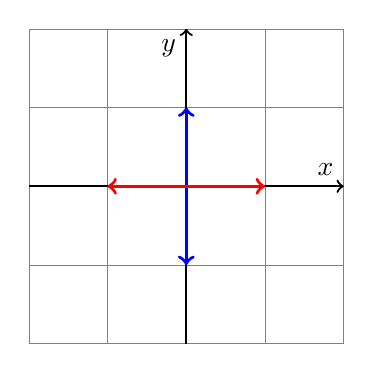
\begin{tikzpicture}
  
  \draw[step=1cm,gray,very thin] (-2,-2) grid (2,2);
  \draw[thick,->] (0,-2) -- (0,2) node[anchor=north, below left] {$y$};
  \draw[thick,->] (-2,0) -- (2, 0) node[anchor=east, above left] {$x$};

  \draw[very thick,->,blue] (0,0) -- (0, 1) node[anchor=east, above left] {};
  \draw[very thick,->,blue] (0,0) -- (0, -1) node[anchor=west, above left] {};
  \draw[very thick,->,red] (0,0) -- (1, 0) node[anchor=north, above left] {};
  \draw[very thick,->,red] (0,0) -- (-1, 0) node[anchor=south, above left] {};

  \end{tikzpicture}
\end{center}


В трёхмерном случае не всё так однозначно. У нас есть шесть направлений. И в данном
случае вероятность возвращения будет строго меньше единицы. С этим разобраться
мы предложим читателю в будущих задачах.

\begin{center}
  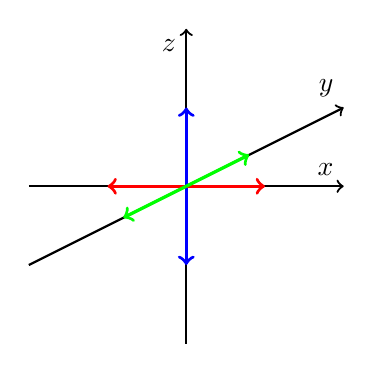
\begin{tikzpicture}
  
  \draw[thick,->] (0,-2) -- (0,2) node[anchor=north, below left] {$z$};
  \draw[thick,->] (-2,0) -- (2, 0) node[anchor=east, above left] {$x$};
  \draw[thick,->] (-2,-1) -- (2, 1) node[anchor=east, above left] {$y$};

  \draw[very thick,->,blue] (0,0) -- (0, 1) node[anchor=east, above left] {};
  \draw[very thick,->,blue] (0,0) -- (0, -1) node[anchor=west, above left] {};
  \draw[very thick,->,red] (0,0) -- (1, 0) node[anchor=north, above left] {};
  \draw[very thick,->,red] (0,0) -- (-1, 0) node[anchor=south, above left] {};
  \draw[very thick,->,green] (0, 0) -- (0.8,0.4) node[anchor=south, above left] {};
  \draw[very thick,->,green] (0, 0) -- (-0.8,-0.4) node[anchor=south, above left] {};


  \end{tikzpicture}
\end{center}

На самом деле всё это зависит от $\Pr{S_{2n} = 0}$. При $d = 1$ и $p = q = \frac{1}{2}$
получим, что $\Pr{S_{2n} = 0} = \binom{2n}{n}4^{-n} \approx \Theta\left(\frac{1}{\sqrt{n}}\right)$, ряд расходится.

При $d = 2$ будет $\Theta\left(\frac{1}{n}\right)$, что тоже расходится, с каждой
новой размерностью добавляется этот самый $\sqrt{n}$ в знаменателе, поэтому
с $d = 3$ ряд будет сходящимся. Это была подсказка на будущие задачи, ничего
тут мы пока не доказывали.

\subsection{Числа Каталана через биномиальные коэффициенты}
Вспомним некоторые факты про ряд Тейлора, а именно, что

\[
  (1 + x)^{\alpha} = \sum\limits_{n = 0}^{+\infty} \binom{\alpha}{n}x^n,
\]

где $\binom{\alpha}{n} = \frac{\alpha(\alpha - 1)\ldots (\alpha - n + 1)}{n!}$.

Поэтому давайте преобразуем ряд для $f(x) = \sum\limits_{n = 0}^{+\infty} C_n x^n$.

\[
  \sqrt{1 - 4x} = \sum\limits_{n = 0}^{+\infty} \binom{1/2}{n}x^n = 
  1 + \sum\limits_{n = 1}^{+\infty} \frac{\frac{1}{2}\left(\frac{1}{2} - 1\right)
  \ldots\left(\frac{1}{2} - n + 1\right)}{n!}(-4x)^n = 
\]

Вынесем $1/2$ из каждой дроби, везде поменяем знак, получим, что это домножится
на $(-1)^{n - 1}$, что совместно с $(-4x)^n$ даст знак минус, в скобках
останется $(2n - 3)!!$:

\[
  = 1 - \sum\limits_{n = 1}^{+\infty} \frac{4^n x^n (2n - 3)!!}{2^n n!} =
  1 - \sum\limits_{n = 1}^{+\infty} \frac{2^n x^n (2n - 3)!!}{n!} = 
\]

Домножим на $n!$ и разделим на него, а также домножим на $2n - 1$ и опять же
разделим. Воспользуемся тем, что $(2n)! = (2n - 1)!! n! \cdot 2^n$:

\[
  = 1 - \sum\limits_{n = 1}^{+\infty} \frac{(2n)!x^n}{n!n!}\frac{1}{2n - 1} =
  1 - \sum\limits_{n = 1}^{+\infty} \binom{2n}{n} \frac{x^n}{2n - 1}
\]

Откуда:

\[
  f(x) = \frac{1}{2x}(1 - \sqrt{1 - 4x}) = \frac{1}{2}\sum\limits_{n = 1}^{+\infty}
  \binom{2n}{n} \frac{1}{2n - 1}x^{n - 1} = 
  \frac{1}{2}\sum\limits_{n = 0}^{+\infty} \binom{2n + 2}{n + 1} \frac{1}{2n + 1}x^{n} =
  \sum\limits_{n = 0}^{+\infty} \binom{2n}{n} \frac{1}{n + 1}x^{n}
\]

В последнем равенстве можно убедиться непосредственно.

Откуда получаем $C_k = \frac{1}{k + 1}\binom{2k}{k}$.

\begin{remark}
  $\Pr{S_1 \neq 0, \ldots, S_{2n - 1} \neq 0, S_{2n} = 0} = 2C_{n - 1}(pq)^n =
  \binom{2n}{n}(pq)^n\frac{1}{2n - 1}$ --- распределение первого момента в нуле.
\end{remark}

\subsection{Математическое ожидание первого момента возвращения в ноль}

\begin{definition}
  $X = \min(2n : S_{2n} = 0)$.
\end{definition}

\begin{theorem}
  $\E{X} = +\infty$.
\end{theorem}

\begin{proof}
  Если $p \neq q$, тогда $\Pr{x = +\infty} > 0$, поэтому матожидание уже
  точно бесконечность.

  Если $p = q = \frac{1}{2}$, тогда $\E{X} = \sum\limits_{n = 1}^{+\infty}
  \Pr{X = 2n}\cdot (2n) = \sum\limits_{n = 1}^{+\infty} \binom{2n}{n} 
  \frac{2n}{2n - 1}\frac{1}{4^n} = \Theta\left(\frac{1}{\sqrt{n}}\right)$, что расходится
\end{proof}

Получается, что да, в ноль мы вернемся, но очень не скоро и бесконечно долго будем
ходить вне. Вот такой вот парадокс. Перейдём к следующему пункту.

\subsection{Среднее время в нуле}

Оказывается, что в нуле мы будем находится не так мало. За $n$ шагов примерно
$\sqrt{n}$ раз мы будем в нуле. Это по большей мере связано с тем, что нули
расположены рядом, то есть есть большая вероятность, что если мы пришли в ноль,
то через малое количество шагов окажемся опять там.

\begin{definition}
  Будем рассматривать симметричное простое случайное блуждание. Тогда 
  $L_n = \left|k : k \in \overline{0, \ldots, n}, S_k = 0\right|$.
\end{definition}

Хотим понять, какая асимптотика у $\E{L_n}$.

\begin{lemma}
  $\E{L_n} = \E{|S_{n + 1}|}$
\end{lemma}

\begin{proof}
  Распишем $|S_{n+1}|$:
  \[
  |S_{n + 1}| =
  \begin{cases}
    1, \text{если $|S_n| = 0$}\\
    S_n + \xi_{n + 1}, \text{если $S_n > 0$}\\
    -S_n - \xi_{n + 1}, \text{если $S_n < 0$}
  \end{cases}
  \]
  Действительно, при положительном $S_n$ мы не поменяем знак, поэтому
  надо лишь добавить то, что мы выбирали на следующем ходу, при отрицательном
  $S_n$ аналогично, а если $S_n = 0$, то в любом случае модуль равен единице.

  Запишем $|S_{n + 1}|$ через индикаторы:

  \[
    |S_{n + 1}| = \I\{|S_n| = 0\} + (S_n + \xi_{n + 1})\I\{S_n > 0\} -(S_n + \xi_{n + 1})\I\{S_n < 0\}
  \]

  Заметим, что $S_n \I\{S_n > 0\} - S_n \I\{S_n < 0\} = |S_n|$ (в этом легко
  убедиться, проверив несколько случаев). Поэтому, введя функцию знака, можно
  утверждать, что:
  \[
   |S_{n + 1}| = \I\{|S_n| = 0\} + |S_n| + \xi_{n + 1}\mathrm{sgn}(S_n)
  \]

  Будем раскрывать рекурсивно, откуда получим:

  \[
    |S_{n + 1}| = \sum\limits_{k = 0}^{n} \I\{|S_k| = 0\} + |S_0| +
    \sum\limits_{k = 0}^{n} \xi_{k + 1}\mathrm{sgn}(S_{k})
  \]

  Заметим, что $L_n = \sum\limits_{k = 0}^{n} \I\{|S_k| = 0\}$, поэтому давайте
  запишем под знаком матожидания с использованием, что $\E{|S_0|} = 0$.

  \[
    \E{|S_{n + 1}|} = \E{L_n} + \sum\limits_{k = 0}^{n} \E{\xi_{k + 1}\mathrm{sgn}(S_{k})}
  \]
  Но величины $\xi_{k + 1}$ и $\mathrm{sgn}(S_{k})$ независимы, так как нет
  пересечений по ходам, поэтому это распадается в произведение матожиданий.

  Ну и финальный аккорд состоит в том, что $\E{\xi_{k + 1}} = 0$, поэтому
  мы доказали равенство.
\end{proof}

Про асимптотику поговорим в следующей лекции.
